% ! TeX root = ../../master-thesis.tex

\section{Unit and Integration Testing}
\label{section:verification:unit-and-integration-testing}

The test suite developed for FRASP consists of around 250 tests, comprising
unit and integration tests, a quarter of which concerns the verification of
aggregate specifications, while the remaining tests verify the infrastructure
built for the evaluation of properties on aggregates, including the simulators,
the extensions for Sodium, and some utilities employed within the library. The
tests have been implemented considering the best practices discussed in Section
\ref{section:analysis:aggregate-convergence-testing} of the analysis,
leveraging the ScalaTest framework \cite{ScalaTest}.

As already anticipated in the analysis, the adopted strategy for verifying the
correctness of the FRASP library is aggregate convergence tests, checking if
the evolution of an aggregate converges towards an expected stable state, given
an aggregate specification and a simulation configuration. Such tests are
modelled by the mixin \texttt{ConvergenceTest} (Figure
\ref{figure:convergent-test-class-diagram}), which can be extended to provide
the inheriting class with methods for creating tests based on convergence,
namely:
\begin{itemize}
  \item \texttt{convergenceTest}: using a provided
        \texttt{ConvergenceSimulator}, check if the evolution of an aggregate
        converges towards (or diverges from) an expected stable state, given an
        aggregate specification and a configuration for the simulation. The
        test can be repeated multiple times for statistical significance, since
        the evolution of the aggregate may be non-deterministic. Additionally,
        a timeout can be set to interrupt the test in case a simulation
        continues indefinitely against expectations (e.g., due to a flaw in the
        implementation of a specification).
  \item \texttt{convergentEquivalenceTest}: similar to
        \texttt{convergenceTest}, but it checks if different aggregate
        specifications converge to the same limit, using the same
        configuration.
\end{itemize}

\begin{figure}[!ht]
  \centering
  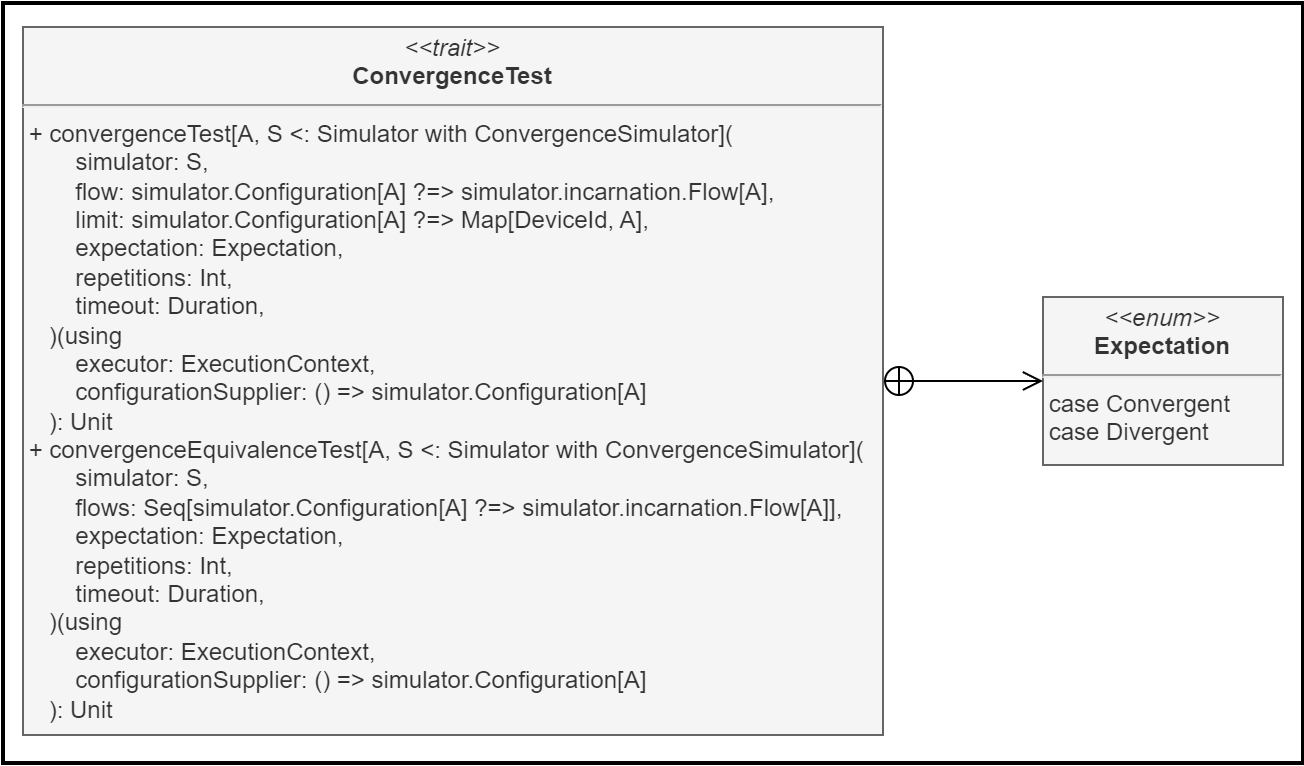
\includegraphics[width=0.8\textwidth]{resources/figures/convergence-test-class-diagram.png}
  \caption{A UML class diagram of the convergent tests.}
  \label{figure:convergent-test-class-diagram}
\end{figure}

In detail, the test suite contains unit \texttt{ConvergenceTest}s, concerning
basic specifications with a single construct, and integration
\texttt{ConvergenceTest}s, concerning more complex specifications with multiple
interacting constructs, including standard aggregate algorithms, such as
gradient-based algorithms. The verified specifications have been collected in a
mixin for \texttt{SimulationIncarnation}, called \texttt{FraspSamples},
granting access to their documentation and declarative names for referencing
them.

\paragraph{Example.}
A practical application of a \texttt{ConvergenceTest} is demonstrated in the
following program (Listing \ref{listing:convergence-test-example}), which
encapsulates all the concepts introduced so far. Note how the test is
essentially a verbose set of initial conditions and an expectation, with no
complex logic at all. Moreover, since the majority of tests share the same
initial conditions, most of the complexity of the configuration can be
eliminated via default parameters, promoting simplicity and standardization.

\lstinputlisting[
  language=Scala,
  caption={
      An application of \texttt{ConvergenceTest}. First, at lines 2-8, the test
      prepares the aggregate computing \ac{DSL}, extended with standard sensors
      (such as the \texttt{Source} sensor) and algorithms (such as the
      \texttt{gradient}). Also, a \texttt{ConvergenceSimulator} is created,
      using the \texttt{StepSimulator} variant. Then, at lines 9-16, all
      simulations are configured to execute in an \texttt{EnvironmentWithTags},
      specifically a grid-like network topology of 25 devices, where the
      $0^{th}$ device is tagged as a source. Additionally, a proper
      \texttt{HaltPolicy} for convergence is selected. Finally, at lines 18-33,
      a concrete convergence test is formulated: the test involves a gradient
      originating from all the devices tagged as sources (i.e., only the
      $0^{th}$ device); the evolution of the aggregate is expected to be
      convergent towards the given limit; and the test is iterated 10 times,
      failing automatically if convergence is not proven within 60 seconds.},
  captionpos=b,
  label={listing:convergence-test-example}
]{resources/listings/convergence-test-example.txt}
